\newpage
\section{Como aplicar Blockchain no contexto de um jogo de vídeo?}
\label{sec:blockchain_how}

Nesta secção é indicada a forma como a tecnologia \textit{blockchain} pode ser aplicada em jogos de vídeo.

\subsection{Mercado Existente}

No mercado de jogos de vídeo, a aplicação de \textit{blockchain}
encontrava-se maioritariamente em jogos que usavam as \acrfullpl{api} do \textit{Ethereum}  e outros com interesses monetários \cite{list_of_blockchain_games} em que os jogos são construídos mais como um casino virtual ou um local de trocas de objetos num mundo virtual com dinheiro real. É disso exemplo o jogo \textit{CryptoKitties} em que houve uma venda de 100 mil dólares por um item do jogo \cite{cryptokitties}, o que não é o tipo de jogo que a \textit{Nerd Monkeys} tem em mente como já explicado na introdução deste capítulo. Para tal começou-se a pensar em implementar algo, à parte, com o objetivo de ser usado exclusivamente como mecanismo de troca de informações entre instâncias do jogo ou jogos caso se queira utilizar a mesma rede entre jogos diferentes.

\subsection{Requerimentos}

Para o desenvolvimento da biblioteca \gamechaining{} existem os seguintes requerimentos:

\begin{itemize}
    \item
          \textbf{R1} - Deve ser agnóstica quanto ao motor de jogo e sistema operativo, isto é, não deve ter quaisquer dependências ou requerimentos que a impeça de ser usada noutras plataformas, exceto se as plataformas em questão forem muito restritas relativamente ao que se pode executar.
    \item
          \textbf{R2} - Deve ser rápida e responsiva, sem grandes requisitos para ser executada, isto é, evitar que use muito do \acrfull{cpu} ou da memória, de forma que não afete muito o desempenho do jogo. Mais especificamente, pretende-se que responda em menos de 10 milissegundos relativamente à chamada de uma função, para não afetar o jogo, exceto se assim for pretendido.
    \item
          \textbf{R3} - Deve ser o mais descentralizada e autónoma possível, o que significa que deve existir o mínimo de manutenção da parte da empresa.
    \item
          \textbf{R4} - Não pode estar presa a licenças comerciais,
          de forma que possa ser de código aberto para uso livre pela comunidade quando assim se pretender.
    \item
          \textbf{R5} - Ser estável e com um design robusto, isto porque, depois de lançado será difícil mudar algo por causa do funcionamento de uma \textit{blockchain}.

\end{itemize}

Estes são os requerimentos que guiam a procura do que é mais apropriado para implementar este projeto, desde a linguagem de implementação, aos algoritmos, arquitetura e à forma como irá interagir com os motores de jogos.

\subsection{Implementação}

Começou-se então a pesquisar sobre como seria desenvolvida essa biblioteca e quais as ferramentas a usar.

\subsection{Desenvolvimento em C++}

\begin{wrapfigure}{l}{2cm}
    \includegraphics[width=2cm]{images/cpp.png}
    \caption{Logótipo de \textit{C++}}
    \label{fig:cpp-logo}
\end{wrapfigure}

A primeira linguagem a considerar para o projeto seria \textit{C++} (\cref{fig:cpp-logo}).
A razão para tal era o seu suporte existente em qualquer plataforma de implementação de jogos, o facto de não ter um \textit{garbage collector}, o código não ser compilado para bytecode ou executado em \textit{runtime}, sendo que em termos de execução o programa seria o mais rápido o possível.

Para o desenvolvimento da biblioteca estudou-se o que seria preciso para criar uma \textit{blockchain} e quais os requesitos, usando como exemplo o \textit{bitcoin} (também implementado em \textit{C++}). Em primeiro lugar, estudou-se o \textit{ZeroMQ}, para a parte de comunicação de rede, que também foi usado no desenvolvimento de \textit{Bitcoin}, e que integrava outros conceitos úteis para o projeto.

\subsubsection{ZeroMQ}
\begin{wrapfigure}{r}{2cm}
    \includegraphics[width=2cm]{images/zeromq/zeromq.png}
    \caption{Logótipo do \textit{ZeroMQ}}
    \label{fig:zeromq-logo}
\end{wrapfigure}

\textit{ZeroMQ}  começou o seu desenvolvimento em 2007 pela iMatix, uma empresa de pesquisa e desenvolve software, para substituir o predecessor \textit{AMQP} \cite{zeromq_origin} e foi anunciado pronto para produção em 2010 \cite{zeromq_mature}. É uma biblioteca de comunicação assíncrona, com o objetivo de ser usada para aplicações concorrentes ou distribuídas.

Em \textit{ZeroMQ} existem tipos especiais de \textit{sockets}, que se ligam a outros tipos compatíveis formando padrões. 

Por exemplo Pedido-Resposta (\cref{fig:zmq_req-rep}), em que se liga um par de \textit{sockets REQ-REP} para que quando um pedido for feito seja fornecida uma resposta, este padrão tem uma relação 1-1, em que um pedido é respondido por uma resposta.

\newpage

\begin{figure}[!ht]
    \centering
    \includegraphics[width=0.25\textwidth]{images/zeromq/req-rep.png}
    \caption{Padrão Pedido-Resposta}
    \label{fig:zmq_req-rep}
\end{figure}

No padrão Publicador-Subscritor, representado na \cref{fig:zmq_pub-sub}, cria-se um \textit{socket} \textit{PUB} e múltiplas \textit{sockets} \textit{SUB}, sendo que quando uma mensagem é enviada pelo PUB é recebida por todas as \textit{sockets SUB}, tendo uma relação 1-X, sendo X um número positivo de publicadores.

\begin{figure}[!ht]
    \centering
    \includegraphics[width=0.55\textwidth]{images/zeromq/pub-sub.png}
    \caption{Padrão Publicador-Subscritor}
    \label{fig:zmq_pub-sub}
\end{figure}

No padrão Pipeline Paralelo, representado na \cref{fig:zmq_pipeline}, usam-se \textit{sockets} PULL e PUSH para melhor distribuição de trabalho. O \textit{Ventilator} envia trabalhos para os trabalhadores e, quando terminados, enviam-se os resultados à \textit{Sink}.

\begin{figure}
    \centering
    \includegraphics[width=0.6\textwidth]{images/zeromq/pipeline.png}
    \caption{Padrão Pipeline Paralela}
    \label{fig:zmq_pipeline}
\end{figure}

Existe também o Pedido-Resposta Estendido, representado na \cref{fig:zmq_req-rep-ext}, em que se estende o padrão Pedido-Resposta para algo mais paralelizado.

\begin{figure}
    \centering
    \includegraphics[width=0.6\textwidth]{images/zeromq/req-rep-ext.png}
    \caption{Padrão Pedido-Resposta Estendido}
    \label{fig:zmq_req-rep-ext}
\end{figure}

Foi seguido o \textit{zguide}, um guia para aprender a usar o \textit{ZeroMQ}, para o estudo destes padrões existindo também explicações para outros padrões mais avançados, como também para fazer aplicações completas utilizando \textit{ZeroMQ}. \cite{zeromq_book}

\clearpage
\subsubsection{Formato dos dados}

Para que seja mais fácil de transferir dados entre implementações e linguagens diferentes deve-se usar um padrão aberto de troca de dados, tanto para ser utilizado através da rede como para comunicar informação entre a biblioteca e os motores de jogos.

Para este problema encontraram-se duas soluções notáveis.

\begin{wrapfigure}{l}{2cm}
    \centering
    \includegraphics[width=2cm]{images/json.png}
    \caption{Logótipo do \acrshort{json}}
    \label{fig:json}
\end{wrapfigure}

A primeira solução consiste em usar \acrfull{json} (\cref{fig:json}). \acrshort{json} é um formato compacto, simples e legível por humanos, é bastante usado e comum em vários sistemas. Muitos motores de jogos e linguagens de programação incluem formas de interagir com este formato, seja com plugins, bibliotecas ou o que pode já estar integrado na ferramenta em questão. O \textit{C++} não integra este aspeto na sua \acrfull{std}, porém, existem múltiplas bibliotecas \textit{online}, de que é exemplo a \textit{json} (mantida por \textit{nlohmann} no \textit{Github} \cite{nlohmann_json}) tendo sido a escolhida por ser entendida como a linguagem mais apropriada.


A segunda solução designada \textit{msgpack} ou \textit{MessagePack} é mantida pela Google. Consiste numa solução equivalente ao \acrshort{json} mas muito mais compacta. \cite{msgpack}. Pode-se visualizar uma comparação entre os dois na \cref{fig:msgpackvsjson}, em que se tem a mesma informação em ambos mas com formatos diferentes, o do topo \acrshort{json}, o de baixo \textit{MessagePack}. A figura explica como a estrutura do \textit{MessagePack} está estruturada e a diferença de tamanhos entre as duas.

\begin{figure}[!ht]
    \centering
    \includegraphics[width=0.8\textwidth]{images/jsonvsmsgpack.png}
    \caption{Comparação entre MessagePack e \acrshort{json} \cite{msgpack}}
    \label{fig:msgpackvsjson}
\end{figure}

Dada a conveniência do formato \acrshort{json} e pelo facto de ser muito mais utilizado e compreensível por humanos decidiu-se escolher esta opção.

\subsubsection{Hashing}

Como o objetivo é fazer uma \textit{blockchain} é necessário conseguir criar \textit{hashs} dos blocos e também útil para outras funcionalidades algorítmicas.

\textit{Hashing} é o processo de dando o mesmo exato conteúdo resulta sempre o mesmo \textit{hash}. Com um \textit{hash} pode se verificar se dados foram modificados ou corrompidos.

Para tal, escolheu-se o \textit{picosha2} como biblioteca de \textit{hashing} com \textit{SHA256}.

\subsubsection{\textit{packaging}}


Recapitulando, já se escolheu \textit{C++} como a linguagem de programação, \textit{ZeroMQ} como a biblioteca para \textit{networking}, \acrshort{json} como o formato de envio de mensagens e \textit{picosha2} para \textit{hashing}.

Com isto já se tem um número considerável de bibliotecas. Em \textit{C++} não existe um gestor de pacotes por predefinição mas existem bastantes possibilidades de escolha como o \textit{vcpkg}, o \textit{conan}, o \textit{hunter} entre outros. No entanto, como nem sempre existem os pacotes que se precisa nestes gestores, pode até haver a necessidade de usar vários ou, o que mais realisticamente acontece, ser o programador a fazer inclusão manual dos pacotes.

Como é previsível que este projeto seja complexo existe a necessidade de um gestor de pacotes para gerir software externo e um gestor do projeto para \textit{packaging}, testes e automatização de \textit{build}. Assim, para este objetivo a escolha óbvia seria o \textit{CMake}. Este gere processos de compilação independentes do compilador a ser usado, testes, verificação de dependências entre outros. Também pode ser integrado com gestores de pacotes como \textit{hunter} que é escrito em CMake e que é fácil de integrar num projeto de CMake o que é o melhor candidato considerando que tem ZeroMQ na sua lista de pacotes, sendo esse o único pacote que não é apenas uma biblioteca \textit{header-only}
\footnote{bibliotecas \textit{header-only} são compostas por apenas ficheiros .h/.hpp em \textit{C/C++}. Estes existem por causa de serem mais fáceis de integrar num projeto mas com o custo de tempos de compilação}.

\subsubsection{Alternativas a considerar}

\textit{C++} é uma óptima linguagem para velocidades de execução e em grande percentagem das plataformas mas poderá ter vários problemas de segurança de memoria, principalmente em aplicações \textit{multithreaded} o que pode aumentar o tempo a depurar o projeto.

\textit{ZeroMQ} é uma boa biblioteca para desenvolver a \textit{networking stack} porém, durante a pesquisa feita, o \textit{libp2p} começou a ser considerada como uma melhor opção. A libp2p é explicada mais abaixo neste documento.

Surgiu assim a ideia de estudar o que outras \textit{blockchains} usavam para desenvolvimento, concluindo-se que a maior parte desta área usava \textit{Go}, uma linguagem de programação simples e relativamente rápida, compilada para código maquina e com um \gls{gc}, fala se mais detalhadamente sobre \textit{Go} na \cref{go}. Porém, encontrou se outra linguagem de desenvolvimento perfeita para os requisitos, \textit{Rust}, resolve muitos dos problemas apresentados sobre o  \textit{C++}.

\subsection{Rust}
\label{subsection:rust}

\textit{Rust} é uma linguagem de programação multi-paradigma compilada projetada para ser "segura, concorrente e prática".
Pode se ver um exemplo da sua sintaxe na \cref{fig:rust-ola}. 
Desenvolvida inicialmente pela \textit{Mozilla} para desenvolver o \textit{Firefox}, isto porque em \textit{C++} e noutras linguagens é difícil de depurar código \textit{multithreaded}. A primeira versão estável de \textit{Rust} foi lançada em 2015. No dia 8 de fevereiro de 2021 foi estabelecida a \textit{Rust Foundation} com a \textit{Amazon}, \textit{Huawei}, \textit{Microsoft}, \textit{Google} e \textit{Mozilla} como fundadores. \cite{rust_wiki}

\begin{figure}[H]
    \centering
    \includegraphics[width=0.8\textwidth]{images/rust-ola.png}
    \caption{Olá Mundo! em \textit{Rust}}
    \label{fig:rust-ola}
\end{figure}

\textit{Rust} tem um gestor de pacotes e projeto integrados, este chamado de \textit{cargo} \cite{cargo_book}, a linguagem compila para código maquina como \textit{C} e \textit{C++} e possui o conceito de \textit{ownership} e \textit{lifetimes} das variáveis integrado na própria linguagem, o que permite detetar com facilidade erros de concorrência e  de \textit{use after deletion}. Adicionalmente, muitas bibliotecas relacionadas com \textit{blockchain} tem implementações desenvolvidas com \textit{Rust}.

Muitas empresas mostram interesse em \textit{Rust}, sendo que este está a ser considerado como a segunda linguagem de programação a ser suportada na \textit{Linux Kernel} e a \textit{Google} utiliza-a para desenvolver novos módulos para \textit{Android} e outros sistemas. Isto porque \textit{Rust} é extremamente seguro. De acordo com estudos 70\% dos \textit{bugs} severos de segurança são causados por problemas de memoria (\cref{fig:memory-errors}) \cite{microsoft_safety} \cite{chromium_safety}. Isto pode parecer um problema que acontece só com linguagens que mexem diretamente com memoria, como o \textit{C} e o \textit{C++} mas isto também se pode  aplicar a \glspl{data-race}
\footnote{\glsdesc{data-race}}.
\textit{Rust} não tem estes problemas face
às suas regras restritas de \textit{ownership}.

\begin{figure}[H]
    \centering
    \includegraphics[width=\textwidth]{images/memory-errors.png}
    \caption{Analise em base de 912 \textit{bugs} de segurança de severidade alta ou crítica desde 2015, que afetavam o canal estável do \textit{Chromium} \cite{chromium_safety}}
    \label{fig:memory-errors}
\end{figure}



\textit{Ownership} funciona com a ideia de que cada espaço de memória, seja este um numérico, uma estrutura ou outro tipo de dados, é propriedade de uma variável. Este espaço de memória pode ser dado a outra variável ou emprestado (borrowed). Uma variável pode ser ou não mutável, isto é, aquando da sua declaração, pode ser definido se o programador consegue ou não mudar o seu valor.

E com estas propriedades é introduzido o  \textit{borrow checker}. Durante a compilação de um programa escrito em \textit{Rust}, o \textit{borrow checker} verifica estas propriedades e a forma como são usadas, provocando erros de compilação caso ocorram condições que podem resultar em \textit{bugs} ou \textit{crashs} provocados por acessos incorretos à memoria. Por exemplo, uma variável que deu posse do seu conteúdo a outra não pode mais ser usada porque não tem conteúdo. Em \textit{Rust}, isto daria um erro de compilação caso fosse tentado, em vez de, na execução, um \textit{segment fault} em \textit{C} e \textit{C++} ou uma \textit{NullException} em linguagens com um \gls{gc} como \textit{Java}.
Com o \textit{borrow checker} também é possível verificar erros relacionados com \glspl{data-race}, o que para acontecer seria necessário que fossem feitos dois acessos à memoria que
\begin{enumerate}
    \item apontassem para a mesma memoria,
    \item estivessem em linhas de execução simultâneas,
    \item pelo menos um fosse uma escrita e 
    \item não estivessem sincronizados.
\end{enumerate}
Porém, o \textit{borrow checker} consegue verificar quando é que as variáveis
\begin{enumerate}
    \item têm acesso à mesma memória,
    \item estão em linhas de execução diferentes,
    \item são mutáveis e
    \item estão sincronizadas
          \footnote{isto é possível com os \textit{traits} \textit{Sync} e \textit{Send} que são detalhes de como \textit{mutexes} e outros estruturas de sincronização são implementadas em \textit{Rust}, dando o contexto necessário ao \textit{borrow checker} \cite{sync_send_traits}}
\end{enumerate}
resultando num erro de compilação quando estas condições ocorressem.

Outras empresas estão a considerar utilizar esta linguagem para projetos em que seja importante a segurança e rapidez, o que reforça a impressão que é uma linguagem que vai ser bem suportada no futuro com novos projetos que noutras circunstâncias usariam \textit{C} ou \textit{C++}.

Depois destes pontos, e considerando o requerimento de estabilidade em R5 decidiu-se usar o \textit{Rust} em vez de \textit{C++}. Sobre as bibliotecas, encontrou-se facilmente \textit{bindings} para \textit{ZeroMQ} e as outras duas bibliotecas tinham alternativas como \textit{sha2} para \textit{hashing} com \textit{SHA-256} e \textit{serde} para serializar e desserializar \acrshort{json}, isto é, transformar as estruturas de \textit{Rust} em \acrshort{json} e vice-versa.


\subsection{Go}
\label{go}
\textit{Go} também foi considerado como outra opção de linguagem de programação a utilizar.
Esta está em grande utilização na implementação de bases de dados em \textit{blockchain} e criptomoedas portanto também se encontram bastantes bibliotecas e exemplos para a implementação das mesmas.

\textit{Go} é uma linguagem feita a pensar em simplicidade com poucas regras de sintaxe e funcionalidades com o objetivo de diminuir o tempo de desenvolvimento e facilitar a sua leitura. Tal como \textit{C} é muito simples de aprender, tem um \gls{gc} para gestão de memoria para que assim o programador não tenha a preocupação de gerir essa memoria.

A razão da escolha de \textit{Rust} em vez de \textit{Go} foi essencialmente devido à sua segurança em termos de gestão de memoria, o que já foi explicado na sub-secção anterior e as seguintes razões:



\begin{itemize}
    \item
          \textit{Rust} não têm um \gls{gc}, a gestão de memória é feita por um conceito chamado \textit{Ownership} parecido com o \gls{raii} em C++, não existindo assim problemas associados ao \textit{\glspl{gc}}.

    \item
          O compilador de \textit{Rust} verifica \textit{data races} em tempo de compilação e erros comuns em que torna o código compilado muito mais seguro, o que evita gastar tempo em depuração e cria programas mais estáveis.

\end{itemize}

\subsection{libp2p}

Durante a pesquisa foi encontrada uma \textit{framework} designada \textit{libp2p} que está a ser desenvolvida em conjunto com o \acrfull{ipfs}
\cite{libp2p_solve}, um protocolo de rede \textit{peer-to-peer} para guardar e partilhar informação num \acrfull{fs} distribuído. \cite{ipfs_wiki}
% Não pode só colocar a referência como sendo o sujeito da frase, assim onde está [21] tem de antes colocar o nome daquilo a que se está a referir.

A \textit{libp2p} foi criada com o objetivo de ajudar a criar aplicações com protocolos de comunicação descentralizados ao contrario do recorrente paradigma de servidor-cliente, que se tem vindo a usar nas ultimas décadas, demonstrando assim uma ótima biblioteca para ajudar no desenvolvimento da aplicação.

\subsection{\acrfull{nat}  \textit{Traversal}}

Um problema que surgiu durante as escolhas de  \textit{networking} foi o de como se iria produzir um jogo completamente descentralizado sem que os utilizadores tivessem a necessidade de "abrir portas" ou fazer outras operações no seu \textit{router} em casa? Isto é um problema com que os utilizadores se deparam com a atual  \textit{Internet}. Dificilmente se faz uma ligação direta entre computadores, sem que existam portas abertas em, pelo menos, um dos lados. Em alguns casos não é possível sem utilizar um \textit{router} alternativo ao que o fornecedor de \textit{Internet} oferece.

Para este problema a solução mais apropriada é \acrshort{nat} \textit{traversal}, isto é uma técnica de estabelecer uma conexão entre \glspl{gateway} que implementam \acrshort{nat} \cite{natt_wiki}.


Estudaram-se algumas técnicas, em especial \textit{hole punching}  \cite{hp_wiki}, usadas em aplicações como \textit{Skype}, \acrfull{voip}, aplicações \acrfull{p2p}, entre outros. \textit{Hole punching} é a ação de, através de um servidor externo com um IP estático público, estabelecer a conexão entre 2 ou mais nós na rede atrás de uma \acrshort{nat}.  \cite{hole_punching}

\textit{Libp2p} também está a desenvolver a sua implementação deste aspeto mas ainda não está finalizado. \cite{natt_lip2p_status}


\subsection{Comunicação}

Para a comunicação entre nós do \gamechaining{} foi considerado o \textit{libp2p}.
Se for usado um serviço externo inicializado quando o jogo inicia ou que esteja constantemente ligado, deve ser feito por \acrfull{ipc-compute} entre o serviço e uma biblioteca que se liga ao jogo apenas para habilitar o jogo a comunicar com o serviço. A biblioteca comunicará com o jogo através de \acrfull{abi}.

O serviço pode ser usado como um servidor que fica conectado constantemente na rede. Este poderia ser comunicado com outras aplicações, não só com instâncias de jogo, como também para verificar valores ou o estado do jogo (com uma interface com o utilizador, caso se queira observar o que está a ocorrer).

Também se pode usar o serviço como um nó para fazer \textit{hole punching} caso assim seja visto como necessário.

As ligações podem ser visualizadas na \cref{fig:gamechaining_coms} em que um cliente (ou nó) liga se a outros nós e ao seu jogo respetivo.

\begin{figure}[!ht]
      \centering
      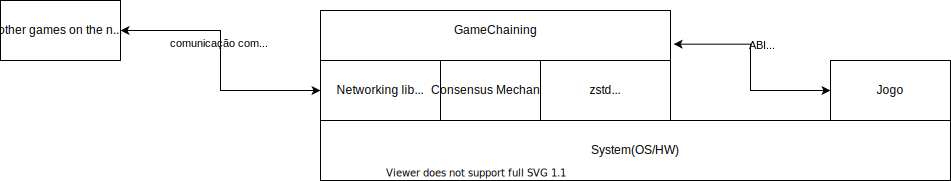
\includegraphics[width=1\textwidth]{blockchain_comunication.png}
      \caption{Comunicações do \gamechaining{}}
      \label{fig:gamechaining_coms}
\end{figure}
